\documentclass
[printout]
% [handout]
{beamer}

\usepackage[utf8]{inputenc}
\usepackage{graphics}
\usepackage{newcent}
\usetheme{Goettingen}
\usecolortheme{beaver}
\title[Git Study Day 1\\Outline]{Outline for Git}
\subtitle{CAT\&DOG Git study 2013\\Day 1}
\author{Eon Jeong}
\date{\today}

\begin{document}

\begin{frame}
  \titlepage
\end{frame}

\setcounter{section}{-1}

\section{Contents}

\begin{frame}{Contents}
  \tableofcontents
\end{frame}

\setcounter{section}{0}

\section{About revision control}

\begin{frame}
  \sectionpage
\end{frame}

\begin{frame}{VCS}
  \textit{\textbf{V}ersion \textbf{c}ontrol \textbf{s}ystem}
  \begin{itemize}
  \item {Or alternatively, \textit{revision control} or \textit{source code control}} \pause
  \item Similar to what you may have experienced as:\begin{description}
  \item[History] 
    features found in wikis or documentations, e.g. Wikipedia\item[Undo/redo]features in most text editors (including even Windows notepad), word processor, spreadsheets, etc.\end{description}
  \end{itemize}
\end{frame}

\begin{frame}{Why do we need a VCS?}
  What if when you are writing a document or a software,
  \begin{itemize}
  \item you are hacked by super mighty 127.0.0.1
  \item then lose everything. :P \pause
  \item or just made a huge wrong modification;
  \item how about writing something together?
  \end{itemize}
  Note that any data or transmission can be very volatile with our electric computers.
\end{frame}

\begin{frame}{What VCS does}
  Assume you are translating an article about something the readers aren't aware of. \pause
  \begin{itemize}
  \item As you have more translations day by day, \pause
  \item some sections should be reviewed later; \pause
  \item some need to be reorganized totally; \pause
  \item some are candidates, now unused but to be merged; \pause
  \item or tomorrow you may want to revert the changes you made today. \pause
  \end{itemize}
  Likewise, development is a hard thing.
  IDEs such as Visual Studio or Eclipse have functions like undo/redo. \textbf{It ain't enough though.}
\end{frame}

\section{Common concepts}

\begin{frame}
  \sectionpage
\end{frame}

\begin{frame}{Repository}
  A typical \textit{version control \textbf{repository}} is whatever includes a historical set of objects (files, folders and references onto them), managed by a VCS. \pause
  \begin{itemize}
  \item Hence, \textit{\textbf{VCS}} is a kind of DBMS around version control operations. \pause(Thus we can assume a good one should follow \textit{ACID}.)\pause
  \item \textit{\textbf{Local}} means the repository or its copy is on the workspace. \pause
  \item \textit{\textbf{Server}} or \textit{\textbf{remote}} means the repository can be accessed via network. \pause
  \item \textit{\textbf{Centralized}} means every client should work on the same repository on a server. \pause
  \item \textit{\textbf{Distributed}} means there are local repository which may have some references to other repos.
  \end{itemize}

\end{frame}

\begin{frame}{Revision}
  A \textit{\textbf{revision}} is the status of contents in the repository at a specific timepoint.\pause
  \begin{itemize}
  \item \textit{\textbf{Commit}} is task making a new revision, or the revision itself. \pause
  \item \textit{\textbf{Checkout}} is task switching the repository to one of its revisions. \pause
  \item \textit{\textbf{Difference}}, or just simply \textit{\textbf{diff}}, is \textit{changeset} between two or more revisions. \pause
  \item \textit{\textbf{Head}} is a reference pointing the last committed (or the last checked out) revision.
  \end{itemize}

\end{frame}

\begin{frame}{Source tree}
  \textit{\textbf{Source tree}}, or \textit{stream}, is the relationship of order among whole revisions of a repository. \pause
  \begin{itemize}
  \item \textit{\textbf{Branch}}, or \textit{codeline}, is a named timeline of revisions with start and end, each is committed on the base of the previous revision of the branch.\pause
  \item \textit{\textbf{Trunk}}, \textit{\textbf{master branch}} or the \textit{mainline} means a unique unnamed branch of the repository. It commonly contains revs from approved diffs.\pause
  \item \textit{\textbf{Merging}} two or more branches cause them share one ongoing revision.\pause
  \item \textit{\textbf{Tag}}, or \textit{label}, is a meaningful snapshot with name, usually a version number. \pause
  \item \textit{\textbf{Fork}} means copying a repo to maintain it independently. The word represents relation among related branches, each having its tail on another branch and its head far forward.
  \end{itemize}
\end{frame}

\begin{frame}{A typical Git 6repository}
  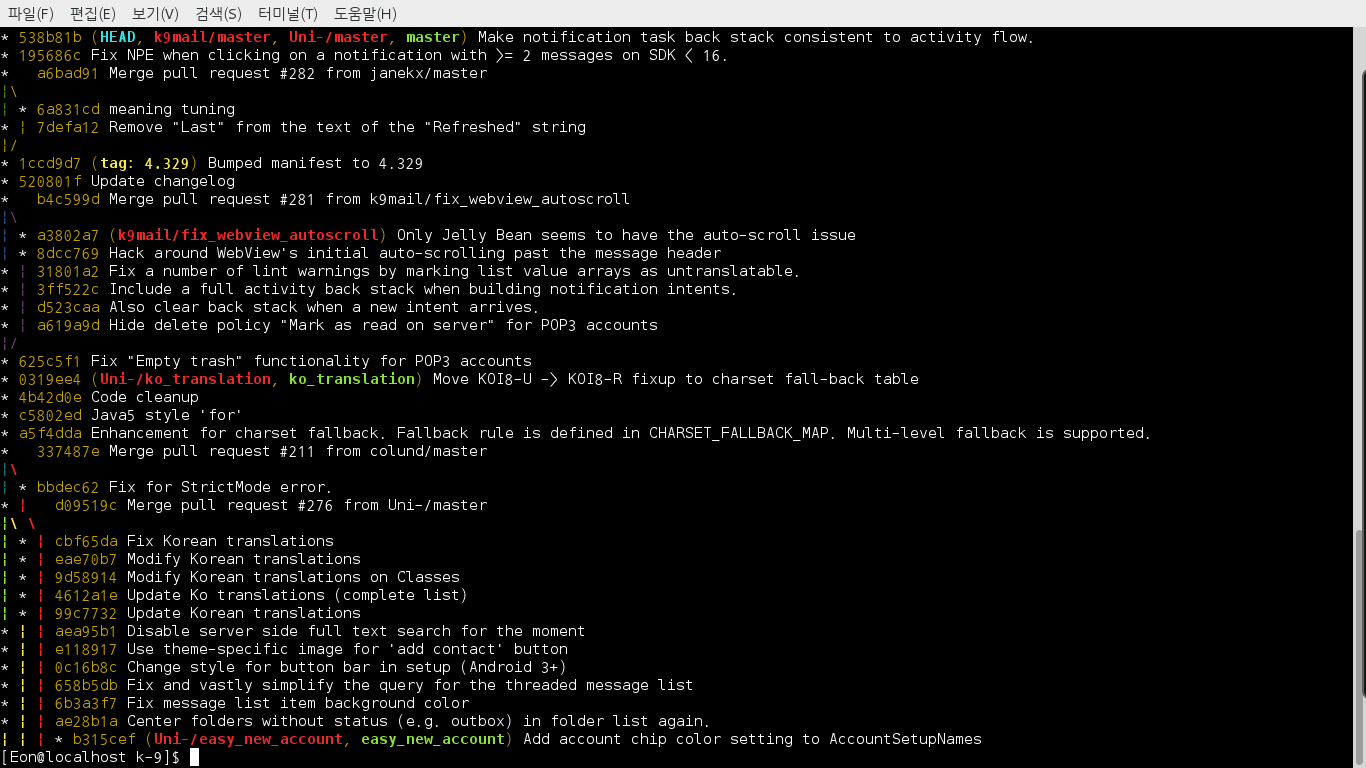
\includegraphics[height=5cm]{repo-example-k9mail.png}\pause
  \begin{enumerate}
  \item \textbf{revision}, diff, head\pause
  \item \textbf{source tree}, branch, merge\pause
  \item ???
  \item PROFIT!
  \end{enumerate}

\end{frame}

\section{About Git}

\begin{frame}
  \sectionpage
\end{frame}

\begin{frame}{Git}
  \begin{flushright}
    
\includegraphics[height=1cm]{git-logo.png}
  \end{flushright}
  \vskip-1cm
  \begin{itemize}
  \item \href{http://git-scm.com}{\underbar{git-scm.com}}\\
  \item Linus Torvalds, 2005 \textasciitilde
  \item written in C, Perl and shell scripts
  \end{itemize}
\end{frame}

\begin{frame}{How to use Git}
  \begin{itemize}
  \item \textit{As-is (I suggest)}
    \begin{itemize}
    \item \texttt{git <command>} in terminal
    \item many direct features associated with software configuration management (SCM) issues
    \item Git is fast!
    \end{itemize}
  \item Or with GUI\  (front-ends)
    \begin{itemize}
    \item \href{http://git-scm.com/downloads/guis}{Git-GUI}
    \item \href{http://www.sourcetreeapp.com/}{SourceTree}
    \item \href{http://www.syntevo.com/smartgithg}{SmartGitHg}
    \item \href{http://windows.github.com/}{GitHub for Windows} (or \href{http://mac.github.com/}{GitHub for Mac})
    \item \href{https://code.google.com/p/tortoisegit}{TortoiseGit}
    \end{itemize}
  \end{itemize}
\end{frame}

\section{Websites}

\begin{frame}
  \sectionpage
\end{frame}

\begin{frame}{GitHub}
  \begin{flushright}
    
\includegraphics[height=1cm]{github-octocat.png}
    
\includegraphics[height=1cm]{github-logo.png}
    \vskip-1cm
    \begin{itemize}
    \item \href{http://github.com}{\underbar{github.com}}\\
    \item 2008 \textasciitilde
    \item free public Git repository for any size of teams
    \item fast fork, pull request, tree graph for forks, issue tracker, wiki
    \item star, watch
    \item 'flavored' markdown
    \item template repository (called Gist)
    \item web page hosting
    \item similar: Gitorious
    \end{itemize}
  \end{flushright}

\end{frame}

\begin{frame}{Bitbucket}
  \begin{flushright}
    
\includegraphics[height=1cm]{bitbucket-logo.png}
    \vskip-1cm
    \begin{itemize}
    \item \href{http://bitbucket.org}{\underbar{bitbucket.org}}\\
    \item 2008 \textasciitilde
    \item free public/private Git/Mercurial repository for small teams
    \item fast fork, pull request, tree graph, issue tracker, wiki
    \item star, fast diff
    \item similar: Launchpad
    \end{itemize}
  \end{flushright}

\end{frame}

\begin{frame}{Others}
  \begin{description}
  \item[\href{http://p.catdog.wo.tc/}{John Mang}] (2010\textasciitilde) supports only SVN, not Git.
  \item[\href{http://code.google.com/}{Google Code}] (2005\textasciitilde) supports Git as well as CVS and Subversion.
  \item[\href{http://sourceforge.net/}{Sourceforge}] (1999\textasciitilde) supports Git, Mercurial, Bazaar, Subversion, CVS.
  \item[\href{http://kldp.net/}{KLDP.net}] (2002\textasciitilde) supports same VCSs as Google code; \href{http://dev.naver.com/}{Naver Developer Center} uses the same engine, nForge.
  \end{description}
\end{frame}

\section{Assignment}

\begin{frame}{First week's assignment}
  \begin{enumerate}
  \item \textbf{Install Git}
    \begin{itemize}
    \item \href{http://msysgit.github.com/}{Get \textit{MSysGit}} to use Git in command line, Windows.
    \item If you want a good GUI, Don't use \textit{TortoiseGit}.
    \end{itemize}
  \item \textbf{Sign up GitHub}
    \begin{itemize}
    \item This is necessary for the upcoming second assignment.
    \end{itemize}
  \end{enumerate}
\end{frame}

\end{document}
